% CVPR 2026 Paper Template; see https://github.com/cvpr-org/author-kit

\documentclass[10pt,twocolumn,letterpaper]{article}

%%%%%%%%% PAPER TYPE
% \usepackage{cvpr}              % To produce the CAMERA-READY version
\usepackage[review]{cvpr}        % To produce the REVIEW version
% \usepackage[pagenumbers]{cvpr} % To force page numbers, e.g. for an arXiv version

%% Editing %%%%%%%%%%%%%%%%%%%%%%%%%%%%%%%%%%%%%%%%%%%%%%%%%%%%%% 
\newcommand{\MIGHTCHANGE}[1]{{\textcolor{magenta}{#1}}}
% \newcommand{\TODO}[1]{{\textbf{\textcolor{todo}{TODO: #1}}}}
% \newcommand{\todo}[1]{\textbf{\textcolor{todo}{#1}}}

%colors
\newcommand{\bgcolor}[2]{\setlength{\fboxsep}{0pt}\colorbox{#1}{\strut #2}}
\newcommand{\BGcolor}[3][HTML]{\definecolor{mycolor}{HTML}{#2}\bgcolor{mycolor}{#3}}

\newcommand{\method}[1]{{NewtPhys}}

%% edits
\newcommand{\FP}[1]{\textcolor{author2}{#1}}
\newcommand{\SC}[1]{\textcolor{author4}{#1}}
\newcommand{\LF}[1]{\textcolor{author1}{#1}}

%% comments
\newcommand{\FPc}[1]{\textcolor{author2}{[\textbf{FP}: #1]}}
\newcommand{\SCc}[1]{\textcolor{author4}{[\textbf{SC}: #1]}}
\newcommand{\LFc}[1]{\textcolor{author1}{[\textbf{LF}: #1]}}


%\renewcommand{\RC}[1]{#1}
%\renewcommand{\SC}[1]{#1}
%\renewcommand{\THV}[1]{#1}
%\renewcommand{\andrei}[1]{#1}
%
%\renewcommand{\RCc}[1]{}
%\renewcommand{\SCc}[1]{}
%\renewcommand{\THVc}[1]{}
%\renewcommand{\andreic}[1]{}
%
%\renewcommand{\todo}[1]{}

%% Colors %%%%%%%%%%%%%%%%%%%%%%%%%%%%%%%%%%%%%%%%%%%%%%%%%%%%%% 
\definecolor{darkmagenta}{RGB}{186, 0, 186}
\definecolor{slateblue}{RGB}{90, 70, 230}

\definecolor{todo}{HTML}{E15554}
\definecolor{author1}{HTML}{40A050}
\definecolor{author2}{HTML}{C33C54}
\definecolor{author3}{HTML}{E6AA68}
\definecolor{author4}{HTML}{0F4893}

\definecolor{material}{HTML}{2BAE27}
\definecolor{mechanics}{HTML}{FF5733}
\definecolor{spatial}{HTML}{3498DB}
\definecolor{permanence}{HTML}{F43FC7}
\definecolor{temporal}{HTML}{0DA792}
\definecolor{viewpoint}{HTML}{EEAC32}

%% Custom macro %%%%%%%%%%%%%%%%%%%%%%%%%%%%%%%%%%%%%%%%%%%%%%%%%%%%%% 
\newcommand{\materialCol}[1]{\textcolor{material}{#1}}
\newcommand{\mechanicsCol}[1]{\textcolor{mechanics}{#1}}
\newcommand{\spatialCol}[1]{\textcolor{spatial}{#1}}
\newcommand{\permanenceCol}[1]{\textcolor{permanence}{#1}}
\newcommand{\temporalCol}[1]{\textcolor{temporal}{#1}}
\newcommand{\viewpointCol}[1]{\textcolor{viewpoint}{#1}}

\newcommand{\material}{\materialCol{material understanding}}
\newcommand{\Material}{\materialCol{Material understanding}}
\newcommand{\mechanics}{\mechanicsCol{mechanics}}
\newcommand{\Mechanics}{\mechanicsCol{Mechanics}}
\newcommand{\spatial}{\spatialCol{spatial reasoning}}
\newcommand{\Spatial}{\spatialCol{Spatial reasoning}}
\newcommand{\permanence}{\permanenceCol{permanence}}
\newcommand{\Permanence}{\permanenceCol{Permanence}}
\newcommand{\temporal}{\temporalCol{temporal reasoning}}
\newcommand{\Temporal}{\temporalCol{Temporal reasoning}}
\newcommand{\viewpoint}{\viewpointCol{viewpoint}}
\newcommand{\Viewpoint}{\viewpointCol{Viewpoint}}


%% Method %%%%%%%%%%%%%%%%%%%%%%%%%%%%%%%%%%%%%%%%%%%%%%%%%%%%%% 
\newcommand{\Enc}{\mathcal{E}}       % Encoder function
\newcommand{\Dec}{\mathcal{D}}       % Decoder function

%% dataset
% \newcommand{\vkitti}{Virtual KITTI 2}
% \newcommand{\vkitti}{VKITTI 2}
% \newcommand{\kittiflow}{KITTI Flow}
% \newcommand{\kitti}{KITTI}
% \newcommand{\diode}{DIODE}
% \newcommand{\hypersim}{Hypersim}
% \newcommand{\flying}{FlyingThings3D}
% \newcommand{\cs}[0]{Cityscapes}


% Abbrv versions
% \newcommand{\SSemantic}{\textbf{\textcolor{semantic}{Seg.}}}
% \newcommand{\NNormal}{\textbf{\textcolor{normal}{Normal}}}
% \newcommand{\DDepth}{\textbf{\textcolor{depth}{Depth}}}
% \newcommand{\OOpticalflow}{\textbf{\textcolor{opticalflow}{Opt.Flow}}}
% \newcommand{\SSceneflow}{\textbf{\textcolor{sceneflow}{Sc.Flow}}}
% \newcommand{\SShading}{\textbf{\textcolor{shading}{Sha.}}}
% \newcommand{\AAlbedo}{\textbf{\textcolor{albedo}{Alb.}}}

%% Abbreviations %%%%%%%%%%%%%%%%%%%%%%%%%%%%%%%%%%%%%%%%%%%%%%%%%%%%%% 
\newcommand{\condenseparagraph}[1]{{\vspace*{0.1em}\noindent\textbf{#1}\quad}}

% Add a period to the end of an abbreviation unless there's one already, then \xspace.
\makeatletter
\DeclareRobustCommand\onedot{\futurelet\@let@token\@onedot}
\def\@onedot{\ifx\@let@token.\else.\null\fi\xspace}

\def\eg{\emph{e.g}\onedot} \def\Eg{\emph{E.g}\onedot}
\def\ie{\emph{i.e}\onedot} \def\Ie{\emph{I.e}\onedot}
\def\cf{\emph{cf}\onedot} \def\Cf{\emph{Cf}\onedot}
\def\etc{\emph{etc}\onedot} \def\vs{\emph{vs}\onedot}
\def\wrt{w.r.t\onedot} \def\dof{d.o.f\onedot}

%% Tables/Figures %%%%%%%%%%%%%%%%%%%%%%%%%%%%%%%%%%%%%%%%%%%%%%%%%%%%%%

\newcommand{\stl}[1]{{\textcolor{gray}{#1}}}


\newcommand{\imgsize}{.125\textwidth}
 
%% centered resized column
%\newcolumntype{C}[1]{>{\centering\let\newline\\\arraybackslash\hspace{0pt}}m{#1}}
%% add spacer between two columns
%\newcolumntype{S}[1]{@{\hspace{#1}}}
%% hide whole column
%\newcolumntype{H}{>{\setbox0=\hbox\bgroup}c<{\egroup}@{}}
%% vertical cell content
\newcommand{\STAB}[1]{\begin{tabular}{@{}c@{}}#1\end{tabular}}
\newcommand{\verti}[2]{\multirow{1}{*}[#1]{\rotatebox[origin=c]{90}{#2}}}

\newcommand{\best}[1]{\textbf{#1}}
\newcommand{\second}[1]{\underline{#1}}

\definecolor{best}{HTML}{C6EFCE}    % light green
\definecolor{second}{HTML}{FFF2CC}  % light yellow
\newcommand{\dataset}[1]{{\scriptsize\textcolor{gray}{#1}}}


%% Annotations %%%%%%%%%%%%%%%%%%%%%%%%%%%%%%%%%%%%%%%%%%%%%%%%%%%%%%
\newcommand{\deltam}{\Delta_{\rm m}}




%% heatmap table
% --- In your preamble ---
% \usepackage[table]{xcolor}
% \usepackage{colortbl}

% 10-step pastel gradient: light red → soft orange → yellow → mint → dark green
\definecolor{pgrade1}{RGB}{255,204,204}  % very light red (worst)
\definecolor{pgrade2}{RGB}{255,221,204}  % light salmon
\definecolor{pgrade3}{RGB}{255,238,204}  % light orange
\definecolor{pgrade4}{RGB}{255,255,204}  % pale yellow
\definecolor{pgrade5}{RGB}{229,255,204}  % yellow-green
\definecolor{pgrade6}{RGB}{204,255,204}  % light mint
\definecolor{pgrade7}{RGB}{178,242,187}  % mint green
\definecolor{pgrade8}{RGB}{153,230,170}  % soft green
\definecolor{pgrade9}{RGB}{102,204,136}  % medium green
\definecolor{pgrade10}{RGB}{51,153,102}  % dark green (best)

% Pastel green → white gradient (strong correlation = green)
\definecolor{corr0}{RGB}{255,255,255}  % white (no correlation)
\definecolor{corr1}{RGB}{229,245,233}
\definecolor{corr2}{RGB}{204,232,207}
\definecolor{corr3}{RGB}{168,221,181}
\definecolor{corr4}{RGB}{123,204,196}
\definecolor{corr5}{RGB}{78,179,211}
\definecolor{corr6}{RGB}{43,140,190}
\definecolor{corr7}{RGB}{29,116,155}
\definecolor{corr8}{RGB}{20,90,120}
\definecolor{corr9}{RGB}{0,68,89}      % dark teal-green (strongest)

\input{preamble}

\definecolor{cvprblue}{rgb}{0.21,0.49,0.74}
\usepackage[pagebackref,breaklinks,colorlinks,allcolors=cvprblue]{hyperref}

\def\paperID{TBD}
\def\confName{CVPR}
\def\confYear{2026}

\title{Few-shot training-free fine-grained semantic segmentation on the FungiTastic Dataset}

\author{Anonymous Authors}

\begin{document}
\twocolumn[{%
\renewcommand\twocolumn[1][]{#1}%
\maketitle
\begin{center}
\begin{minipage}[t]{0.49\textwidth}
    \centering
    \small\textbf{Teaser A. Oracle masks on 200 classes: DINOv3 backbone vs.\ descriptor.}

    \vspace{0.35em}

    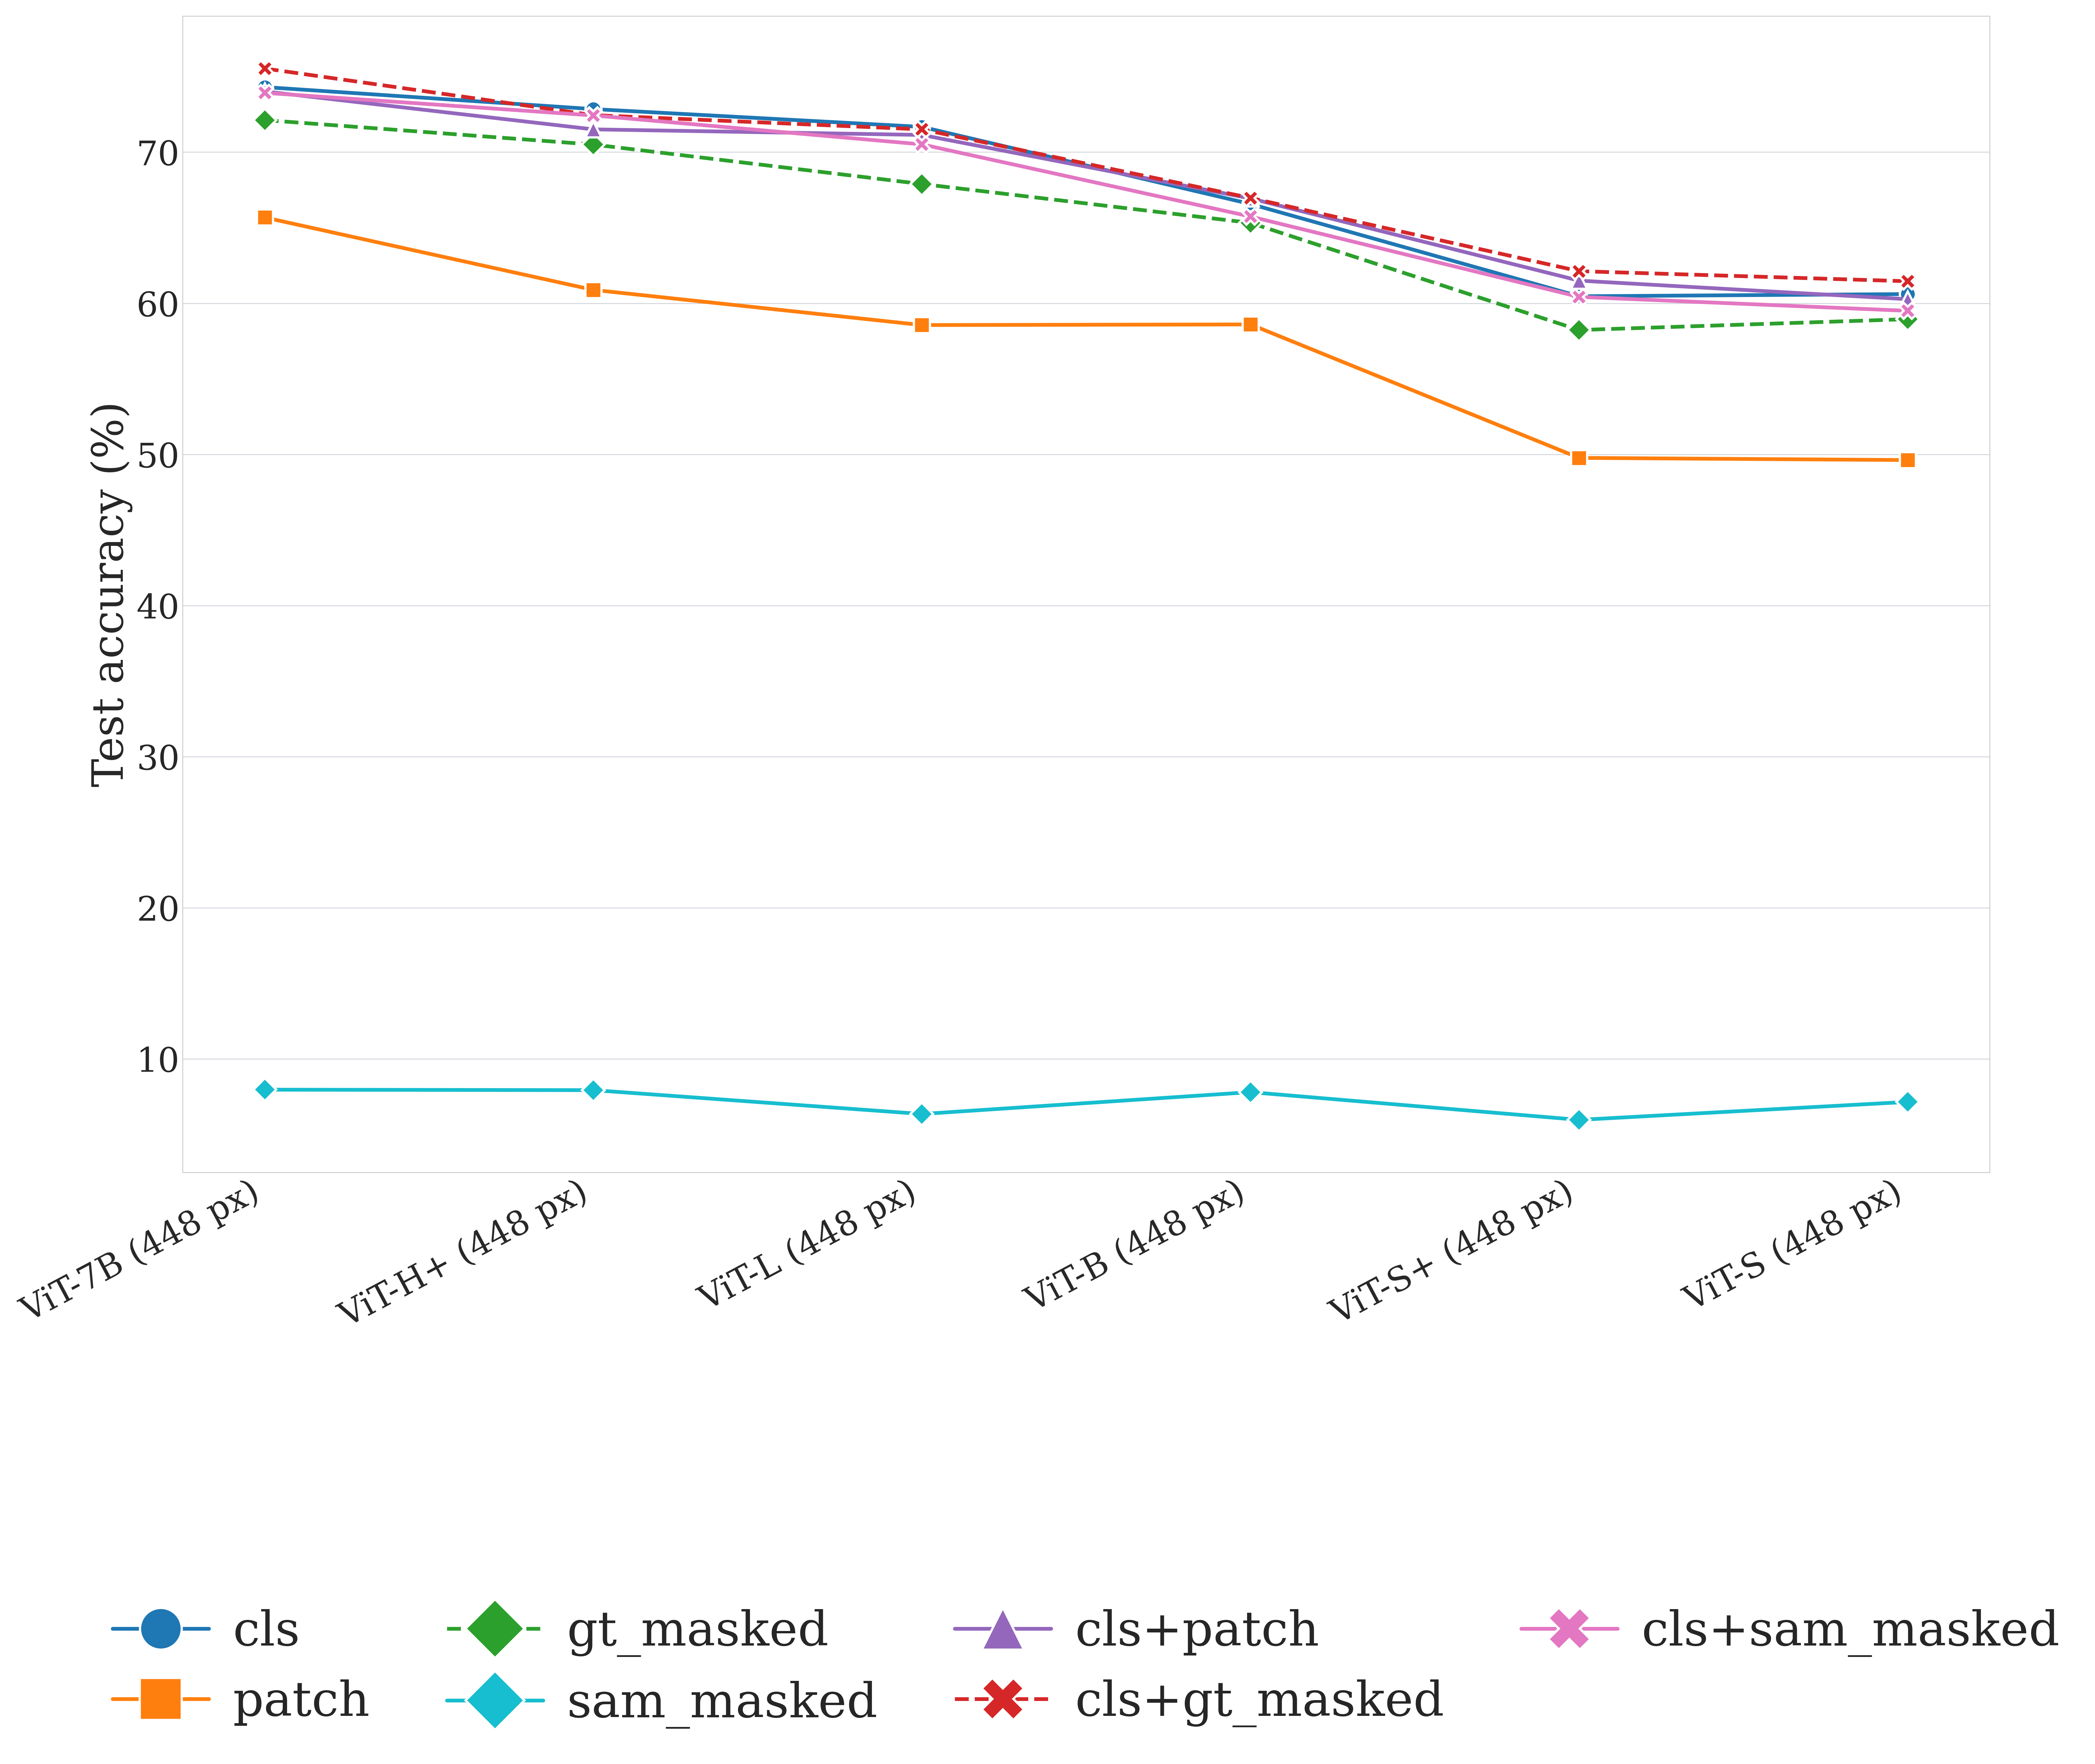
\includegraphics[width=\linewidth]{media/teaser/mlp_absolute_test_acc_sorted.png}

    \vspace{0.15em}

    \footnotesize Accuracy rises with backbone scale, and \texttt{cls+masked} is strongest throughout.
\end{minipage}
\hfill
\begin{minipage}[t]{0.49\textwidth}
    \centering
    \small\textbf{Teaser B. SAM-3 on 2000 classes: DINOv3 backbone vs.\ descriptor.}

    \vspace{0.35em}

    \includegraphics[width=\linewidth]{example-image}

    \vspace{0.15em}

    \footnotesize Reserved slot for the 2000-class SAM-3 teaser; final plot export is pending.
\end{minipage}

\vspace{0.4em}

\captionsetup{type=figure}
\caption{Top-line teaser layout matching the repo README. Teaser A is now populated with the exported oracle-mask comparison across the DINOv3 suite under a fixed MLP head, while Teaser B keeps the planned 2000-class SAM-3 slot visible until those runs are exported.}
\label{fig:teaser}
\end{center}

\vspace{0.6em}
}]
\begin{abstract}
We study whether oracle foreground masks improve feature-based fine-grained fungal recognition when strong frozen visual features are already available. On a 215-class closed-set subset of FungiTastic, we extract frozen DINOv3 ViT-7B descriptors and compare seven token constructions at `224' and `448' resolution: CLS, mean pooled patches, mask-aware pooled patches, and simple concatenations of global and local features. All variants are evaluated with the same small MLP classifier to isolate the effect of the representation. We find that masks help most when used as a complementary local cue rather than as a standalone descriptor. Fusing the CLS token with mask-aware pooled patches gives the best accuracy at both resolutions, reaching \textbf{74.04}\% at `224' and \textbf{75.53}\% at `448', improving over plain CLS by 1.82 and 1.23 points, respectively. In contrast, naive mean pooling over all patches is consistently weak, and branch-wise input normalization does not help. These results suggest that, for frozen fungal features, oracle masks are most useful for refining local evidence while preserving global context.
\end{abstract}

\section{Introduction}

Fine-grained fungal recognition is difficult for the same reasons that make many ecological benchmarks interesting: species can be visually similar, the class distribution is long-tailed, and the background often contains strong clutter. FungiTastic extends earlier Danish fungi benchmarks with a much broader multi-modal dataset, including expert-verified labels, metadata, and segmentation masks for a subset of images \cite{Picek_2022_WACV,picek2022automatic,picek2024fungitastic}. This creates a clean question for the current repo: if we already have strong frozen visual features, when do oracle masks still help?

The answer is not obvious. A foreground mask can suppress irrelevant background and isolate shape-sensitive regions, but it can also remove context that remains useful for recognition. The practical choice is therefore not just \emph{with mask} versus \emph{without mask}; it is also \emph{which token representation should receive the mask signal}, and whether that signal should replace or complement the global image representation.

This draft focuses on the narrowest version of that question. We keep the backbone fixed, keep the background augmentation fixed, and vary only token construction and image resolution. Specifically, we compare CLS-only, full patch pooling, mask-aware patch pooling, and simple feature concatenations at `224' and `448' resolution. Every variant is trained with the same small MLP on frozen features, so the comparison isolates representation quality rather than end-to-end backbone adaptation.

The completed runs already support three takeaways:
\begin{itemize}[leftmargin=*]
\item Oracle masks are most useful as a complement to global context, not as a standalone descriptor.
\item Patch-only mean pooling is substantially weaker than CLS-based representations at both resolutions.
\item Higher resolution improves absolute accuracy, but the marginal gain from mask fusion does not increase in the completed runs.
\end{itemize}

The rest of the paper documents this first result slice and makes the current state of the project buildable and reviewable.

\section{Related Works}

\paragraph{Fine-grained learning in low-data regimes.}
Fine-grained learning under limited supervision has been studied mainly for classification. The survey in \cite{tang2024awesome_fgfs} shows that prior work is largely restricted to image-level recognition, with little attention to dense prediction. Fine-grained semantic segmentation is more demanding, as it requires both recognition and precise localization. Only a small number of recent works, such as \cite{part_matching}, address related settings, mainly through part-level correspondence rather than category-level segmentation.

\paragraph{FungiTastic benchmark and prior solutions.}
FungiTastic \cite{Picek_2025_CVPR} has so far been explored mostly for classification. Recent FungiCLEF submissions, such as \cite{prototypical_networks, contrastive}, focus on long-tailed recognition through feature engineering, ensembling, and lightweight finetuning. These methods target classification and do not address fine-grained segmentation.

\paragraph{Prototype-based methods.}
Prototype-based learning is a standard approach for few-shot recognition \cite{proto1, proto2, proto3}, where classes are represented in an embedding space. Recent works also use multimodal prototypes to improve generalization under class imbalance \cite{multimodal}. Our method follows this idea, but combines prototype-based classification with class-agnostic segmentation in a single pipeline.

\paragraph{PCA whitening and feature preprocessing.}
PCA whitening is a common preprocessing step for distance-based inference, as it decorrelates features and normalizes variance across directions \cite{kessy2018optimal}. It is particularly useful when pretrained embeddings are dominated by nuisance variation rather than task-relevant structure \cite{anthony2026invisible, weng2022investigation}. This makes it a natural choice for prototype matching in our setting.
\section{Experimental Setup}
\label{sec:setup}

\begin{figure}[t]
    \centering
    
\includegraphics[width=\linewidth]{../FungiTastic/assets/img/Figure1-observation.png}
    \caption{FungiTastic observations combine images, expert-verified labels, and segmentation masks for a subset of the data \cite{picek2024fungitastic}. Our study uses the binary foreground mask only to compute mask-aware mean pooling over ViT patch tokens.}
    \label{fig:fungitastic}
\end{figure}

\paragraph{Data.}
The current closed-set experiments operate on extracted features for 215 classes. According to the saved run metadata, the effective split contains 19,077 training samples, 3,368 internal validation samples, and 9,763 test samples. The training code first loads the extracted \texttt{train} and \texttt{val} feature folders, concatenates them, and then creates a new stratified 85/15 train/validation split for early stopping. The held-out \texttt{test} features remain untouched.

\paragraph{Frozen features.}
All experiments use frozen DINOv3 ViT-7B features extracted once per image. For each sample, the extraction pipeline stores three descriptors: the global CLS token, the mean of all patch tokens, and a mask-aware mean of patch tokens where the patch weights come from the binary foreground mask. We evaluate two image resolutions, `224' and `448', under the default \texttt{normal} background setting.

\paragraph{Feature variants.}
The token study compares seven inputs to the classifier:
\texttt{cls},
\texttt{patch},
\texttt{masked},
\texttt{cls+patch},
\texttt{cls+patch\_norm},
\texttt{cls+masked},
and \texttt{cls+masked\_norm}.
The normalized variants apply per-branch $\ell_2$ normalization before fusion.

\paragraph{Classifier.}
Each feature branch is projected to 256 dimensions with a linear layer followed by ReLU. The projected branches are concatenated, passed through a 512-dimensional hidden layer, and mapped to 215 output classes. Optimization uses AdamW with learning rate $3 \times 10^{-4}$, weight decay $10^{-4}$, batch size 64, and a maximum of 200 epochs. Early stopping monitors validation loss with patience 30 and minimum improvement $10^{-4}$. The seed is fixed to 7 for all runs.

\paragraph{Metric.}
The current dashboard tracks top-1 accuracy, so that is the metric reported in this draft. Additional metrics such as macro accuracy and stratified scores are planned in the repo but are not yet available for the completed runs.

\section{Results}
\label{sec:results}

\begin{table*}[t]
    \centering
    \small
    \setlength{\tabcolsep}{8pt}
    \begin{tabular}{lccc}
        \toprule
        Feature variant & `224' test acc. (\%) & `448' test acc. (\%) & $\Delta_{448-224}$ \\
        \midrule
        \texttt{cls} & 72.22 & 74.30 & +2.08 \\
        \texttt{patch} & 64.40 & 65.68 & +1.28 \\
        \texttt{masked} & 72.05 & 72.12 & +0.07 \\
        \texttt{cls+patch} & 71.97 & 74.01 & +2.05 \\
        \texttt{cls+patch\_norm} & 71.06 & 73.27 & +2.20 \\
        \texttt{cls+masked} & \textbf{74.04} & \textbf{75.53} & +1.49 \\
        \texttt{cls+masked\_norm} & 72.41 & 73.02 & +0.61 \\
        \bottomrule
    \end{tabular}
    \caption{Top-1 test accuracy for the completed MLP token study. Oracle mask information is most effective when fused with the global CLS token.}
    \label{tab:main-results}
\end{table*}

\paragraph{Mask fusion is the best completed configuration.}
\Cref{tab:main-results} shows a clear winner: \texttt{cls+masked} is the best feature variant at both resolutions. Relative to plain \texttt{cls}, mask fusion improves top-1 test accuracy by 1.82 points at `224' and 1.23 points at `448'. Relative to \texttt{cls+patch}, the gain is 2.08 points at `224' and 1.52 points at `448'. This supports the practical view that masks are useful primarily as an additional local cue on top of a strong global descriptor.

\paragraph{Masked pooling alone is not enough.}
The \texttt{masked} variant does not beat \texttt{cls} at either resolution. At `224' it is nearly tied with \texttt{cls}, but at `448' it falls more than two points behind. This suggests that the mask helps suppress irrelevant regions, yet the global image summary still carries important context that should not be discarded.

\paragraph{Naive patch pooling is consistently weak.}
The \texttt{patch} variant is the worst model in both settings, reaching only 64.40\% at `224' and 65.68\% at `448'. Even adding patch pooling to CLS without masks does not improve over \texttt{cls} alone. The likely interpretation is that averaging all spatial tokens mixes useful foreground details with background clutter and dilutes the strongest discriminative evidence.

\paragraph{Higher resolution helps absolute accuracy, but not the relative mask gain.}
Moving from `224' to `448' improves nearly every variant, and the best absolute score comes from \texttt{cls+masked} at `448'. However, the gain of \texttt{cls+masked} over \texttt{cls} shrinks from 1.82 to 1.23 points. In other words, the completed runs support \emph{higher resolution helps}, but they do not support the stronger claim that \emph{masks help more at higher resolution}.

\paragraph{Input normalization is not beneficial here.}
Both normalized fusion variants underperform their unnormalized counterparts. For this small MLP setup, simple raw feature concatenation is the stronger default.

\section{Discussion}

\paragraph{What the current evidence says.}
The completed experiments suggest a simple answer to the paper question. Oracle masks help when they refine local evidence without replacing the global representation. The strongest recipe is therefore not ``mask-only'', but ``CLS plus mask-aware pooled patches''. This is a useful negative result as well: access to an oracle foreground mask does not automatically justify discarding the original global token.

\paragraph{Why patch-only pooling fails.}
The largest gap in \Cref{tab:main-results} is between CLS-based descriptors and plain patch averaging. That gap is too large to ignore. It indicates that a naive spatial mean is a poor summary for this task, likely because fungal images often include distractors such as leaves, soil, wood, or multiple overlapping structures. Oracle masks partially correct that issue, but only the fused representation preserves enough global context to turn the correction into a consistent win.

\paragraph{Current limitations.}
This draft intentionally reports only what is already completed in the repo. The evidence is limited to one backbone, one classifier family, one random seed, one background mode, and one metric. Prototype, k-NN, and linear-probe baselines are still pending. Stratified analyses by class frequency, mask area, and hard species pairs are also still blocked. As a result, the current paper should be read as a first reproducible slice of the project rather than a finished benchmark study.

\paragraph{Immediate next steps.}
The next experiments are clear from the dashboard plan: add non-parametric and linear baselines, measure whether the same ranking survives with lower-capacity classifiers, and then stratify the gains to identify which examples benefit most from oracle masks. That follow-up is necessary before making stronger claims about representation quality or ecological failure modes.

\section{Conclusion}

The current result slice gives a concrete answer. On frozen DINOv3 fungal features, oracle masks help most when they are fused with the CLS token, not when they replace it. The best completed model, \texttt{cls+masked}, reaches 74.04\% top-1 accuracy at `224' and 75.53\% at `448'. Higher resolution improves the absolute score, but the relative advantage of masks does not increase. This makes the current story for the repo precise and buildable: \emph{oracle masks are complementary local evidence, and simple token fusion is already enough to expose that effect.}

{
    \small
    \bibliographystyle{ieeenat_fullname}
    \bibliography{main}
}

\end{document}
